%%%%%%%%%%%%%%%%%%%%%%%%%%%%%%%%%%%%%%%%%%%%%%%%%%%%%%%%%%%%%%%%%%%%%%%%%%%%%%%%
% Preámbulo                                                                    %
%%%%%%%%%%%%%%%%%%%%%%%%%%%%%%%%%%%%%%%%%%%%%%%%%%%%%%%%%%%%%%%%%%%%%%%%%%%%%%%%

 
\documentclass[11pt,a4paper,titlepage,twoside,openright,openbib]{report}
%%% RELACIÓN DE VARIABLES A PERSONALIZAR %%%
\def\lingua{eng}
%\def\lingua{esp} % descomenta esta liña se redactarás a memoria en español
%\def\lingua{eng} % descomenta esta liña se redactarás a memoria en inglés
\def\nome{Adrián Rodríguez Louzán}                             % substitúe aquí o teu nome
\def\nomedirectorA{Francisco Javier Taibo Pena}             % substitúe aquí o nome de quen dirixe
\def\nomedirectorB{ Emilio José Padrón González}
\def\nomedirectorC{ Luis Omar Álvarez Mures}
\def\titulo{IMPLEMENTATION OF AN AUTOMATIC CAMERA OPERATOR USING DEEP REINFORCEMENT LEARNING} % substitúe aquí o título do teu TFG
%\def\mencion{NOME DA MENCIÓN}                        % descomenta a mención correspondente
\def\mencion{COMPUTACIÓN}
%\def\mencion{ENXEÑARÍA DO SOFTWARE}
%\def\mencion{ENXEÑARÍA DE COMPUTADORES}
%\def\mencion{SISTEMAS DE INFORMACIÓN}
%\def\mencion{TECNOLOXÍAS DA INFORMACIÓN}

%\def\renomearcadros{si} % descomenta esta liña se redactas a memoria en español e prefires que
                         % os "cuadros" e o "índice de cuadros" se renomeen
                         % a "tablas" e "índice de tablas" respectivamente

\usepackage{estilo_tfg}

% Lista de paquetes potencialmente interesantes (uso baixo demanda)

% \usepackage{alltt}       % proporciona o entorno alltt, semellante a verbatim pero que respecta comandos
% \usepackage{enumitem}    % permite personalizar os entornos de lista
% \usepackage{eurofont}    % proporciona o comando \euro
% \usepackage{float}       % permite máis opcións para controlar obxectos flotantes (táboas, figuras)
% \usepackage{hhline}      % permie personalizar as liñas horizontais en arrays e táboas
% \usepackage{longtable}   % permite construir táboas que ocupan máis dunha páxina
% \usepackage{lscape}      % permite colocar partes do documento en orientación apaisada
% \usepackage{moreverb}    % permite personalizar o entorno verbatim
% \usepackage{multirow}    % permite crear celdas que ocupan varias filas da mesma táboa
% \usepackage{pdfpages}    % permite insertar ficheiros en PDF no documento
% \usepackage{rotating}    % permite diferentes tipos de rotacións para figuras e táboas
% \usepackage{subcaption}  % permite a inclusión de varias subfiguras nunha figura
% \usepackage{tabu}        % permite táboas flexibles
% \usepackage{tabularx}    % permite táboas con columnas de anchura determinada

%%%%%%%%%%%%%%%%%%%%%%%%%%%%%%%%%%%%%%%%%%%%%%%%%%%%%%%%%%%%%%%%%%%%%%%%%%%%%%%%
% Corpo                                                                        %
%%%%%%%%%%%%%%%%%%%%%%%%%%%%%%%%%%%%%%%%%%%%%%%%%%%%%%%%%%%%%%%%%%%%%%%%%%%%%%%%

\begin{document}

 %%%%%%%%%%%%%%%%%%%%%%%%%%%%%%%%%%%%%%%%
 % Preliminares do documento            %
 %%%%%%%%%%%%%%%%%%%%%%%%%%%%%%%%%%%%%%%%

 \begin{titlepage}
  
  \hspace*{128pt}
  \textcolor{udcpink}{{\fontencoding{T1}\fontfamily{phv}\selectfont Facultade de Informática}}\\[-32pt]

  \begin{center}
    
\includegraphics[scale=0.3]{imaxes/udc}\\[35pt]

    {\large TRABALLO FIN DE GRAO \\
            GRAO EN ENXEÑARÍA INFORMÁTICA \\
            MENCIÓN EN \mencion } \\[100pt]
    
    \begin{huge}
      \begin{spacing}{1.3}
        \bfseries \titulo
      \end{spacing}
    \end{huge}
  \end{center}
  
  \vfill
  
  \begin{flushright}
    {\large
    \begin{tabular}{ll}
      {\bf Estudante:} & \nome \\
      {\bf Dirección:} & \nomedirectorA \\ % COPIA E PEGA ESTA LIÑA MÁIS VECES SE O PRECISAS
       & \nomedirectorB \\ % COPIA E PEGA ESTA LIÑA MÁIS VECES SE O PRECISAS
       & \nomedirectorC \\ % COPIA E PEGA ESTA LIÑA MÁIS VECES SE O PRECISAS
    \end{tabular}}
  \end{flushright}
  \rightline{A Coruña, \datasimple\today.}
\end{titlepage}

 \paxinaenbranco
 \dedicatoria{To my family and my brother} % escribe neste comando o teu texto de dedicatoria
 \paxinaenbranco
 \paxinaenbranco
 \begin{agradecementos}
First of all, I would like to thank my family for supporting me unconditionally and placing all their trust in me.\\
Thanks also to my friends, those that I made during this 4 years,
but even more to those who I met during my internation experience in South Korea.\\
Finally, I want to give my gratitude to my project managers Francisco Javier Taibo Pena, Emilio José Padrón Gonzalez and Luis Omar Álvarez Mures, without whom I could not have carried out this project. Thank you for all your attention.               % substitúe este comando polo teu texto de agradecementos
 \end{agradecementos}
 \paxinaenbranco
 %%%%%%%%%%%%%%%%%%%%%%%%%%%%%%%%%%%%%%%%%%%%%%%%%%%%%%%%%%%%%%%%%%%%%%%%%%%%%%%%

\begin{abstract}\thispagestyle{empty}
El aprendizaje por refuerzo (AR) es un área del aprendizaje automático que se ocupa de cómo los agentes software deben tomar acciones en un entorno para maximizar alguna noción de recompensa acumulativa. \\
Los problemas de interés en el aprendizaje por refuerzo también se han estudiado en la teoría del control óptimo,
que se ocupa principalmente de la existencia y caracterización de soluciones óptimas y algoritmos para su
cálculo exacto, y menos con aprendizaje o aproximación, particularmente en ausencia de un modelo matemático
del medio ambiente. Los algoritmos de refuerzo que incorporan el aprendizaje profundo pueden vencer a los campeones mundiales en el Juego de Go, así como expertos humanos que juegan numerosos videojuegos de Atari. \\

En este proyecto, aprovecharemos el aprendizaje de refuerzo profundo y los motores de juego para modelar una escena deportiva típica y enseñarle a un agente a capturar la acción con la cámara. Primero, una escena que se asemeja a un partido deportivo será creado utilizando el motor de juego elegido. A continuación, probaremos diferentes algoritmos de aprendizaje por refuerzo profundo.
 % substitúe este comando polo resumo do teu TFG
             % na lingua principal do documento (tipicamente: galego)

  \vspace*{25pt}
  \begin{segundoresumo}
 Reinforcement learning (RL) is an area of machine learning concerned with how software agents ought to take
 actions in an environment so as to maximize some notion of cumulative reward. \\ 
 The problems of interest in reinforcement learning have also been studied in the theory of optimal control,
 which is concerned mostly with the existence and characterization of optimal solutions, and algorithms for their
 exact computation, and less with learning or approximation, particularly in the absence of a mathematical model
 of the environment. Reinforcement algorithms that incorporate deep learning can beat world champions at the
 game of Go as well as human experts playing numerous Atari video games.\\
 In this project, we will leverage Deep Reinforcement Learning and game engines to model a typical sports scene
 and teach an agent to capture the action on camera. First, a scene which resembles a sports match will be
 created using the chosen game engine. Next, we will test out different Deep Reinforcement Learning algorithms. % substitúe este comando polo resumo do teu TFG
               % na lingua secundaria do documento (tipicamente: inglés)
  \end{segundoresumo}
\vspace*{25pt}
\begin{multicols}{2}
\begin{description}
\item [\palabraschaveprincipal:] \mbox{} \\[-20pt]
  \begin{itemize}
  	\item Inteligencia Artificial
  	\item Deep Reinforcement Learning
  	\item Operador de cámara
  	\item DQN
  	\item Python
  	\item Tensorflow
  	\item Keras
  \end{itemize}	 % substitúe este comando por un itemize
                         % que relacione as palabras chave
                         % que mellor identifiquen o teu TFG
                         % no idioma principal da memoria (tipicamente: galego)
\end{description}
\begin{description}
\item [\palabraschavesecundaria:] \mbox{} \\[-20pt]
  \begin{itemize}
	\item Artificial Intelligence
	\item Deep Reinforcement Learning
	\item Camera operator
	\item DQN
	\item Python
	\item Tensorflow
	\item Keras
\end{itemize}% substitúe este comando por un itemize
                         % que relacione as palabras chave
                         % que mellor identifiquen o teu TFG
                         % no idioma secundario da memoria (tipicamente: inglés)
\end{description}
\end{multicols}

\end{abstract}

%%%%%%%%%%%%%%%%%%%%%%%%%%%%%%%%%%%%%%%%%%%%%%%%%%%%%%%%%%%%%%%%%%%%%%%%%%%%%%%%

 \paxinaenbranco

 \pagenumbering{roman}
 \setcounter{page}{1}
 \bstctlcite{IEEEexample:BSTcontrol}

 \tableofcontents
 \listoffigures
 \listoftables
 \cleardoublepage
 
 \pagenumbering{arabic}
 \setcounter{page}{1}

 %%%%%%%%%%%%%%%%%%%%%%%%%%%%%%%%%%%%%%%%
 % Capítulos                            %
 %%%%%%%%%%%%%%%%%%%%%%%%%%%%%%%%%%%%%%%%

 \chapter{Introdución}
\label{chap:introducion}

%\lettrine{P}{rimer} capítulo da memoria, onde xeralmente se exporán as
%liñas mestras do traballo, os obxectivos, etc. Incluimos un par de
%exemplos de citas~\cite{ErlangBook,ErlangWebBook} e de referencias
%internas (sección \ref{sec:mostra}, páxina \pageref{sec:mostra}).

Deep Reinforcement Learning (DRL), a very fast-moving field, is the combination of Reinforcement Learning and Deep Learning and it is also the most trending type of Machine Learning at this moment because it is being able to solve a wide range of complex decision-making tasks that were previously out of reach for a machine to solve real-world problems with human-like intelligence.\\
In this introduction I will try to explain the fundamentals and concepts around Artificial intelligence and Machine Learning, in order to then deeply dive into our program and how I implemented it.\\
\subsection{Artificial Intelligence and Machine Learning}
We can divide Artificial Intelligence into two categories \textbf{Narrow AI} and \textbf{General A.I.}

\begin{figure}[htbp]
	\centering
	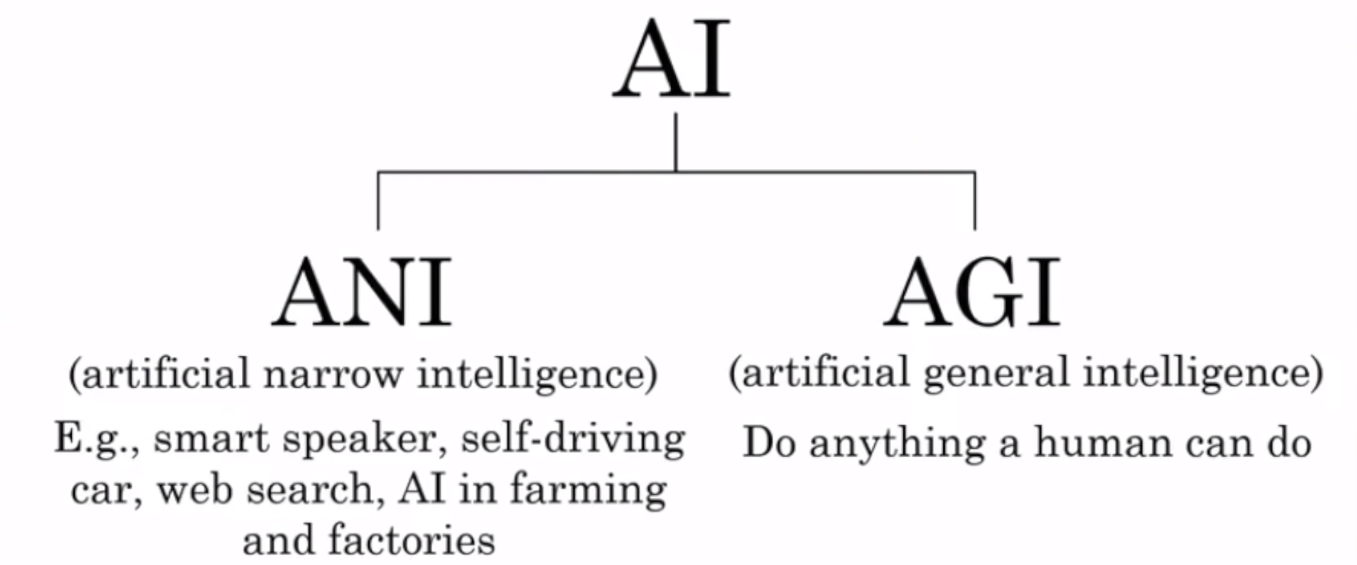
\includegraphics[scale=0.25]{imaxes/cattegories_AI.png}
	\caption{Categories of Artificial Intelligence}
	\label{categoriesAI}
\end{figure}

Most of the movies and representations that we see in the mainstream media are around General A.I. Machines that do everything that humans do, and better. It can talk, it can learn to play games, it can communicate... etc \\
Right now, in our field we are working on narrow A.I. Are machines that can do only one thing and the application of the machine is narrowed to a specific goal. In this field and in the recent years, great advances were made.For instance, AlphaGo defeated the best professional human player in the game of Go. Or last year, for instance, our friend Oriol Vinyals and his team in DeepMind showed the AlphaStar agent beat professional players at the game of StarCraft II. Or a few months later, OpenAI?s Dota-2-playing bot became the first AI system to beat the world champions in an e-sports game.\\

Machine Learning ~\cite{ml4dummies} is one of the many approaches that Artificial Intelligence (AI) uses when it comes to extracting knowledge from experience, not only as a tool to
achieve the objectives linked to AI but as a vehicle to reduce time and effort
used for resolution. ML recognizes patterns through the use of examples in
rather than addressing its implementation. The machine learns a model from examples and
use this one to solve the problem. A system that continuously learns, that is capable of
make decisions based on data instead of algorithms and that changes your behavior, it is a system based on ML.
Given a problem the choice of the appropriate algorithm is not trivial. For this it is necessary
ask yourself two fundamental questions: what do I want to do? and what information
I have to achieve my goal? Both require us to carry out an exhaustive analysis of the
own problem and the data, quantity and quality, that we have for its resolution.

\begin{figure}[hp!]
	\centering	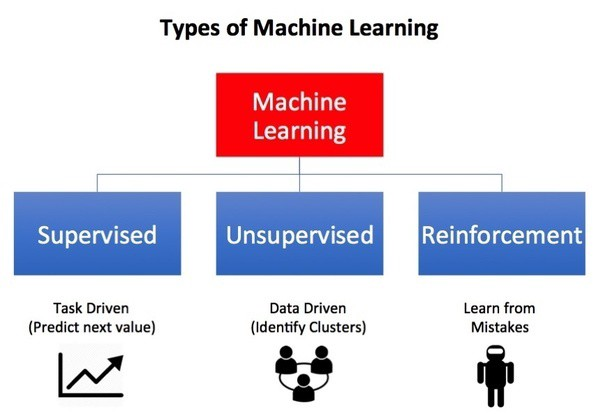
\includegraphics[scale=0.50]{imaxes/machine_learning.jpeg}
	\caption{Types of Machine Learning}
	\label{fig:ml_types}
\end{figure}


Reinforcement Learning is one of the three branches in which ML techniques are generally categorized:

\begin{itemize}
	\item \textbf{Supervised Learning}is the task of learning from tagged data and its goal is to generalize.
	\item \textbf{Unsupervised Learning}is the task of learning from unlabeled data and its goal is to compress.
	\item \textbf{Reinforcement Learning} is the task of learning through trial and error and its goal is to act.
\end{itemize}

Orthogonal to this categorization we can consider a powerful recent approach to ML, called \textbf{Deep Learning (DL)}, topic of which we have discussed extensively in previous posts. DL is not a separate branch of ML, so it?s not a different task than those described above. DL is a collection of techniques and methods for using neural networks to solve ML tasks, either Supervised Learning, Unsupervised Learning, or Reinforcement Learning and we can represent it graphically in the following figure:

\begin{figure}[htbp]
	\centering
	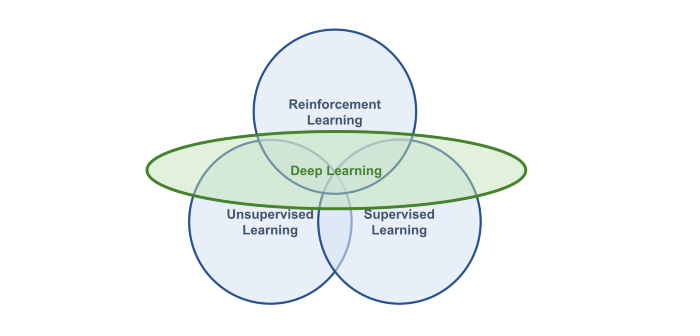
\includegraphics[scale=0.50]{imaxes/deep_learning.png}
	\caption{Visual relationship of Deep Learning with the Machine Learning categories.}
	\label{mlcategories}
\end{figure}


Reinforcement learning ~\cite{reinfLearning}~\cite{introReinf} is a form of machine learning in which an agent attempts to
learn a policy that maximizes a numeric reward signal~\cite{introReinf}. In reinforcement learning,
an agent learns by trial and error and discovers optimal actions through its own experiences. Unlike supervised learning, the agent does not learn by comparing its own actions to those of an expert; everything it learns is from its own interactions with the environment. Reinforcement learning attempts to solve optimization problems that are
defined by a Markov Decision Process (MDP) ~\cite{introReinf}. A A Markov Decision Process defines
the behavior of the environment by mathematically defining the environment´s one step dynamics.\\


%%%%%%%%%%%%%%%%%%%%%%%%%%%%%%%%%%%%%%%%%%%%%%%%%%%%%%%%%%%%%%%%%%%%%%%%%%%%%%%
\subsection{Background for RL.}
%%%%%%%%%%%%%%%%%%%%%%%%%%%%%%%%%%%%%%%%%%%%%%%%%%%%%%%%%%%%%%%%%%%%%%%%%%%%%%%

Markov decision process. MDPs and their multiple variants (e.g., Partially Observable MDP or POMDP) ~\cite{puterman} have been proposed to represent and solve sequential decision-making problems under uncertainty.



%%%%%%%%%%%%%%%%%%%%%%%%%%%%%%%%%%%%%%%%%%%%%%%%%%%%%%%%%%%%%%%%%%%%%%%%%%%%%%%
\subsection{Elements in Reinforcement Learning}
%%%%%%%%%%%%%%%%%%%%%%%%%%%%%%%%%%%%%%%%%%%%%%%%%%%%%%%%%%%%%%%%%%%%%%%%%%%%%%%
In Reinforcement Learning there are two core components:
\begin{itemize}
	\item \textbf{An Agent}, that represents the "solution" , which is a computer program with a single role of making decisions (actions) to solve complex decision-making problems under uncertainty.
	\item \textbf{An Enviroment}, that is the representation of a "problem", which is everything that comes after the decision of the Agent. The environment responds with the consequences of those actions which are observations or states and rewards also sometimes called costs.
\end{itemize}



For example, let´s take the game of PacMan where the goal of the agent(PacMan) is to eat the food in the grid while avoiding the ghosts on its way. In this case, the grid world is the interactive environment for the agent where it acts. Agent receives a reward for eating food and punishment if it gets killed by the ghost (loses the game). The states are the location of the agent in the grid world and the total cumulative reward is the agent winning the game.

\begin{figure}[htbp]
	\centering
	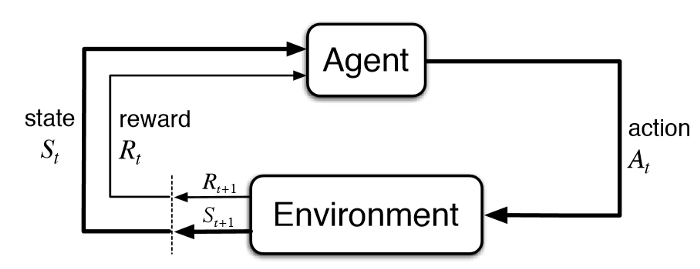
\includegraphics[scale=0.40]{imaxes/rl_agentenv.png}
	\caption{Reinforcement learning cycle}
\end{figure}


These two core components interact constantly in a way that the Agent attempts to make some changes in  the Environment through actions, and the Environment changes due to the Agent?s actions. How the environment changes to certain actions is defined by a model which may or may not be known by the Agent.\\


When the Agent does not know the model, it needs to make decisions with incomplete information; do model-free RL or try to learn the model explicitly as part of the algorithm.\\

\textbf{State}\\
The Environment is represented by a set of variables related to the problem. This set of variables and all the possible values that they can take are referred to as the state space. A state is, a snapshot of the current situation in the enviroment, with all the maximum information about it. In our case, since we had to make our own enviroment, it will be define by the frame of the video and the position of the ball and camera.\\

\textbf{Observation}\\
Due that we are considering that the Agent doesn?t have access to the actual full state of the Environment, it is usually called observation the part of the state that the Agent can observe. We also followed this convention in order to make it as close as possible to openAI Gym enviroments


\textbf{Action}\\
At each state, the Environment has available a set of actions, from which the Agent will choose. The Agent acts on the Environment through these actions and the Environment may change states as a response to the action taken by the Agent. The function that is responsible for this mapping is called transition function or transition probabilities between states.\\

In our case the action will consist in one of the 5 options in order to move the camera, which are: up, down, right, left, and no-action.


\textbf{Reward}\\
The Environment has a defined task that the agent need to complete, then the Enviroment provide to the Agent a reward signal as a direct answer to the Agent?s actions. This reward is a feedback of how well the last action is contributing to achieve the task to be performed in the Environment. The Agent?s goal is to maximize the overall reward it receives and so rewards are the motivation the Agent needs in order to act in a desired behavior.

\textbf{Episode}\\
The task the Agent is trying to solve may or may not have a natural ending. Tasks that have a natural ending, such as a game, are called episodic tasks. In our case the episodes correspond to a frame in the video, and our agent has to constantly act in the enviroment, that is, continously moving the camera around, the only end is when we reach the last frame of the video.\\

\textbf{Return}\\
As we will see, Agents may take several time steps and episodes to learn how to solve a task. The sum of rewards collected in a single episode is called a return. Agents are often designed to maximize the return.
One of the limitations are that these rewards are not disclosed to the Agent until the end of an episode, what we introduced earlier as ?delayed reward?. For example, in the game of tic-tac-toe the rewards for each individual movement (action) are not known until the end of the game. It will be a positive reward if the agent won the game (because the agent had achieved the overall desired outcome) or a negative reward (penalties) if the agent had lost the game.

%%%%%%%%%%%%%%%%%%%%%%%%%%%%%%%%%%%%%%%%%%%%%%%%%%%%%%%%%%%%%%%%%%%%%%%%%%%%%%%
\subsection{Exploration vs Exploitation}
%%%%%%%%%%%%%%%%%%%%%%%%%%%%%%%%%%%%%%%%%%%%%%%%%%%%%%%%%%%%%%%%%%%%%%%%%%%%%%%

Another important characteristic, and challenge in Reinforcement Learning, is the trade-off between ''exploration'' and ''exploitation''. Trying to obtain a lot of rewards, an Agent must prefer actions that it has tried in the past and knows that will be effective actions in producing reward. But to discover such actions, paradoxically, it has to try actions that it has not selected never before.\\

In order to achieve this in our agent we create a variable called epsilon, that will decay until we reach certain minimum value, the agent will get a random float number in the half-open interval [0.0, 1.0) so that if that number is bigger than epsilon, it will take a random action, else the agent will continue with the action with the highest reward.\\


%%%%%%%%%%%%%%%%%%%%%%%%%%%%%%%%%%%%%%%%%%%%%%%%%%%%%%%%%%%%%%%%%%%%%%%%%%%%%%%
\subsection{Q-Learning}
%%%%%%%%%%%%%%%%%%%%%%%%%%%%%%%%%%%%%%%%%%%%%%%%%%%%%%%%%%%%%%%%%%%%%%%%%%%%%%%
Q-Learning is a model-free form of machine learning, in the sense that the Agent does not need to know or have a model of the environment that it will be in. The same algorithm can be used across a variety of environments.


%\section{Sección de mostra}
%\label{sec:mostra}



%\subsection{Subsección de mostra}


 \chapter{Contido demostrativo}
\label{chap:demo}

\lettrine{E}{ntre} a introdución e as conclusións, o documento conterá
tantos capítulos como sexa preciso, sempre con coidado de non rebasar
o límite de 80 páxinas fixado polo regulamento de TFGs.

Empregaremos éste de xeito demostrativo, para ilustrar o uso de
elementos habituais que poidan ser de utilidade.

\section{Inclusión de imaxes}

Se precisamos imaxes no noso documento, incluirémolas do xeito que se
indica na figura~\ref{fig:exemplo} (páxina~\pageref{fig:exemplo}). Se
o facemos así, \LaTeX ubicará cada imaxe no mellor lugar posible,
lugar que pode variar a medida que o documento vaia crecendo coa
inclusión de máis texto e outros elementos (máis imaxes, táboas,
etc.).

\begin{figure}[hp!]
  \centering
  
\includegraphics[width=0.75\textwidth]{imaxes/udc.png}
  \caption{Pé de imaxe descritivo}
  \label{fig:exemplo}
\end{figure}

Recoméndase almacenar os ficheiros gráficos no directorio
\texttt{imaxes}.

\subsection{Inclusión de varias sub-imaxes}

Se precisamos inserir imaxes relacionadas, pode ser apropiado
incluílas como sub-figuras, do xeito que se pode apreciar na
figura~\ref{fig:exemplo-subfiguras} coas
imaxes~\ref{fig:subfigura-rotada}
e~\ref{fig:subfigura-deformada}. Como se pode ver nos exemplos desta
sección, sempre é recomendable referirse ás imaxes pola súa
referencia, xa que dese xeito non dependemos de onde queden ubicados
os elementos en cuestión.

\begin{figure}[hp!]
  \centering
  \begin{subfigure}[c]{0.3\textwidth}
    
\includegraphics[angle=45,width=\textwidth]{imaxes/udc.png}
    \caption{Pé de subimaxe rotada}
    \label{fig:subfigura-rotada}
  \end{subfigure}
  \hspace{0.1\textwidth}
  \begin{subfigure}[c]{0.3\textwidth}
    
\includegraphics[width=\textwidth,height=3cm]{imaxes/udc.png}
    \caption{Pé de subimaxe deformada}
    \label{fig:subfigura-deformada}
  \end{subfigure}
  \caption{Pé de imaxe xeral}
  \label{fig:exemplo-subfiguras}
\end{figure}

\section{Inclusión de código fonte}

Se precisamos incluír fragmentos de código fonte, podemos facelo da
seguinte maneira:

\begin{lstlisting}[language=C]
#include <stdio.h>
#define N 10

int main()
{
  int i;

  // Isto é un comentario
  puts("Ola, mundo!");

  for (i = 0; i < N; i++)
  {
    puts("LaTeX é a ferramenta de edición ideal para profesionais da informática!");
  }

  return 0;
}
\end{lstlisting}

\section{Uso da relación de acrónimos e do glosario}

Os acrónimos edítanse no ficheiro \texttt{bibliografia/acronimos.tex}
e úsanse empregando a orde \texttt{acrlong} para obter o termo
completo (deste xeito: \acrlong{erlang}), a orde \texttt{acrshort}
para obter o acrónimo (deste xeito: \acrshort{erlang}). A primeira vez
que usamos un termo con acrónimo no documento é recomendable usar orde
\texttt{acrfull} (que produce ambas versións á vez:
\acrfull{erlang}). Os acrónimos que non se usan no documento, non
aparecen na relación que se xerar na versión PDF.

Pola súa banda, os termos do glosario edítanse no ficheiro
\texttt{bibliografia/glo\-sa\-rio.tex} e úsanse empregando a orde
\texttt{gls} (deste xeito, \gls{bytecode}) ou \texttt{Gls} (deste
xeito, \Gls{bytecode}). Ao igual que os acrónimos, os termos que non
se usan no documento, non aparecen na relación que se xera na versión
PDF.

%\include{contido/...}
 \chapter{Conclusións}
\label{chap:conclusions}

\lettrine{D}{erradeiro} capítulo da memoria, onde se presentará a
situación final do traballo, as leccións aprendidas, a relación coas
competencias da titulación en xeral e a mención en particular,
posibles liñas futuras,\dots

\Blindtext


 %%%%%%%%%%%%%%%%%%%%%%%%%%%%%%%%%%%%%%%%
 % Apéndices, glosarios e bibliografía  %
 %%%%%%%%%%%%%%%%%%%%%%%%%%%%%%%%%%%%%%%%

 \appendix
 \appendixpage
 \chapter{Material adicional}
\label{chap:adicional}

\lettrine{E}{xemplo} de capítulo con formato de apéndice, onde se pode
incluír material adicional que non teña cabida no corpo principal do
documento, suxeito á limitación de 80 páxinas establecida no
regulamento de TFGs.

\Blindtext

%\include{anexos/...}

 \printglossary[type=\acronymtype,title=\nomeglosarioacronimos]
 \printglossary[title=\nomeglosariotermos]

 \bibliographystyle{IEEEtran}
 \bibliography{\bibconfig,bibliografia/bibliografia}
 \cleardoublepage
 
\end{document}

%%%%%%%%%%%%%%%%%%%%%%%%%%%%%%%%%%%%%%%%%%%%%%%%%%%%%%%%%%%%%%%%%%%%%%%%%%%%%%%%
